\documentclass{beamer}

\usetheme{Ilmenau}
\usepackage{graphicx}
\usepackage[style=alphabetic]{biblatex}
\usecolortheme{beaver}

\addbibresource{biblio.bib}

\title{Gestor VME}
\institute[Colombia]{Universidad Central}
\date{Febrero 7, 2024}
\author{Odín Santiago Arango Sanchez,
Felipe Medina González y
Juan David Hernández Palomino}
\logo{

\includegraphics[width=1cm]{./pictures/uc.png}
}

\begin{document}
\begin{frame}
  \titlepage
\end{frame}
\begin{frame}{Problemática}
    \framesubtitle{Actores}
    \begin{itemize}
        \item Un sistema (activo TI) tolerante de fallos \parencite{rodriguez} \pause
        \item Las personas que usan en la labor un activo TI \pause
        \item El entorno \pause
        \item Las condiciones en las que se encuentran tales equipos \pause
    \end{itemize}
\end{frame}
\begin{frame}{Problemática}
    \framesubtitle{Situaciones}
    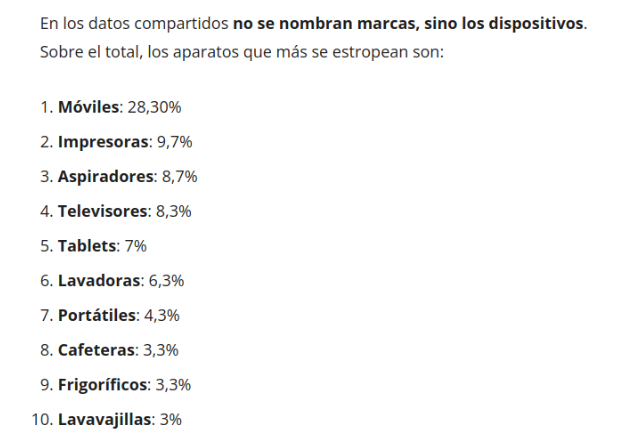
\includegraphics[height=1\textheight]{./pictures/statistics.png}
\end{frame}
\begin{frame}{Problemática}
    \framesubtitle{Situaciones}
    \begin{center}
        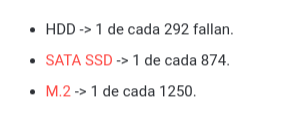
\includegraphics[width=0.6\textwidth]{./pictures/hardware.png} \\
        Esto ocurre según lo que muestra la página de ASUS
    \end{center}
\end{frame}
\begin{frame}{Espina de pescado}
    \begin{center}
        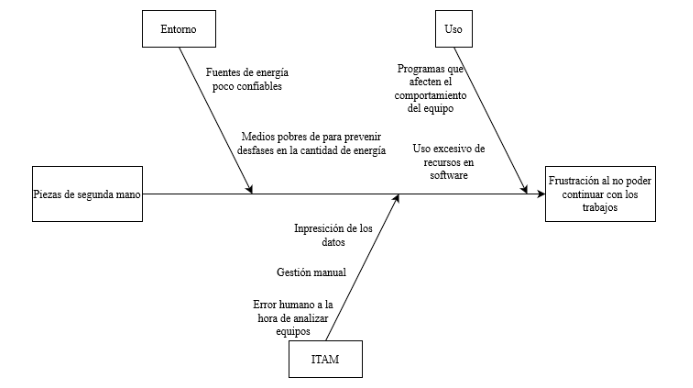
\includegraphics[width=.9\textheight]{./pictures/ishikawa_1.png} \\
        Esta es la que se empleó para el documento de practicas I
    \end{center}
\end{frame}
\begin{frame}{Espina de pescado}
    \begin{center}
        
\includegraphics[width=.9\textheight]{./pictures/ishikawa_2.png}\break
        Esta es la última mejora
    \end{center}
\end{frame}
\input{objectives}
\input{solution}
\begin{frame}
    De acuerdo con \textcite{montaje}, cada elemento del PC es
    diferente pese a sus similitudes, por lo que el software ha
    de saber cómo comunicarse con esos componentes.
\end{frame}
\begin{frame}{Referencias}
    \printbibliography
\end{frame}
\end{document}
